\documentclass[]{standalone}
\usepackage[utf8]{inputenc}
\usepackage{graphicx}
\usepackage[american]{circuitikz}
\usetikzlibrary{arrows,shapes,calc,positioning}

\begin{document}

\pgfmathsetmacro\circuitheight{5}
\pgfmathsetmacro\circuitwidth{4}
\pgfmathsetmacro\mmpos{1.5*\circuitwidth}


\begin{circuitikz}[scale=1]
  \node (mm) at (\mmpos,3) {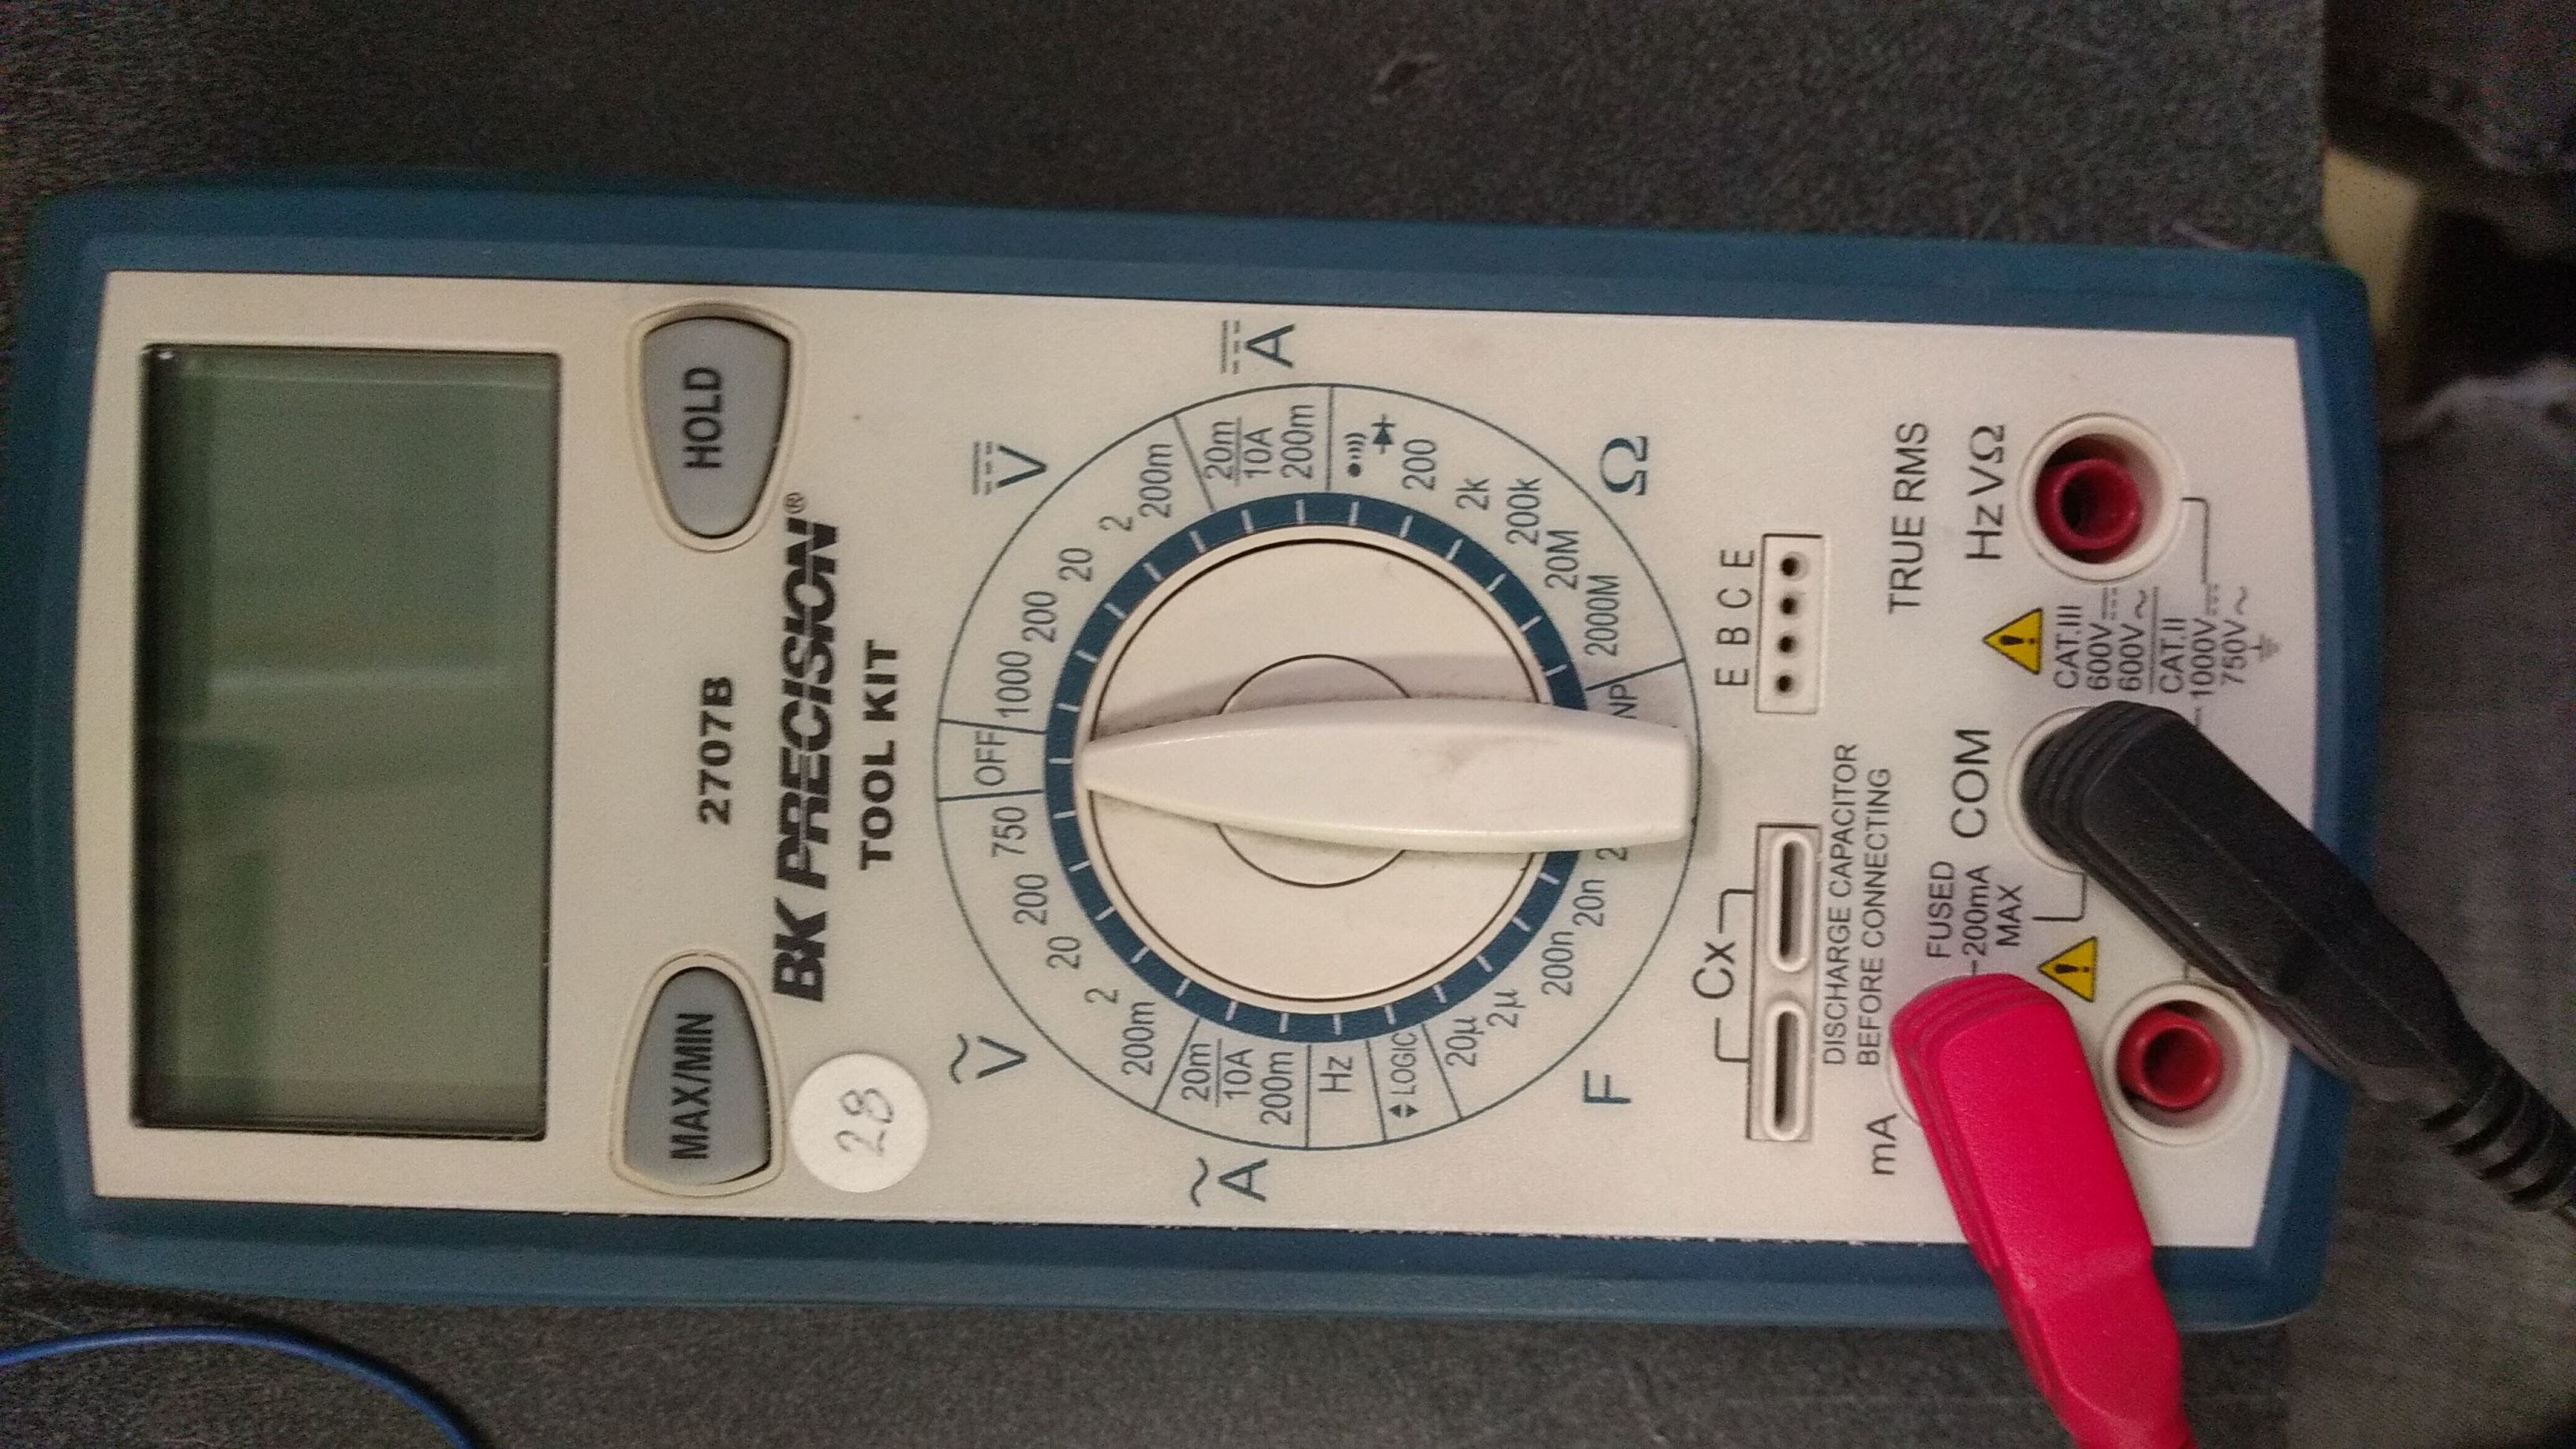
\includegraphics[width=4cm, angle=270]{multimeter-amp.jpg}};
  \node[coordinate] (plus) at ($(mm) + (-1.1,-1.3)$) {};
  \node[coordinate] (minus) at ($(mm) + (-0.7,-1.9)$) {};
  \draw (0,0) to[american voltage source, label=5V] (0, \circuitheight) 
  to[R=$R$,] ++(\circuitwidth,0) node[coordinate] (cp) {};
  \draw[red, ultra thick] (cp) to[out=0, in=180] (plus);
  \draw[black, ultra thick] (minus) to[out=220, in=0] (0,0);
\end{circuitikz}
\end{document}
